\section{Evaluation}\label{sec:eval}

We developed \( \tool \) as an open source tool\footnote{The URL of the tool is
anonymized due to a double-blind review process.}, and evaluated the tool
based on the following three research questions:
\begin{itemize}[leftmargin=0.5cm]
\item RQ1. \textbf{Coverage:} How much parts \( \tool \) automatically extract
the syntax and semantics from ES7 to ES10?
\item RQ2. \textbf{Check with Tests:} The syntax and semantics of the latest
version on ECMAScript (ES10) is compatible with official tests?
\item RQ3. \textbf{Forward Compatibility:} Is \( \tool \) applicable to language
features ready for inclusion in the next ECMAScript (ES11)?
\end{itemize}


\subsection{Coverage}

\begin{table}[t]
  \caption{Number of productions in specifications,
from \textit{all} of which \( \tool \) automatically generated parsers}
  \label{fig:syntax-all-version}
\vspace*{-1em}
\small
  \[
    \begin{array}{c?r|r|r|r?r}
      \textbf{Version}
      & \multicolumn{1}{c|}{\textbf{ES7}}
      & \multicolumn{1}{c|}{\textbf{ES8}}
      & \multicolumn{1}{c|}{\textbf{ES9}}
      & \multicolumn{1}{c?}{\textbf{ES10}}
      & \multicolumn{1}{c}{\textbf{avg.}}\\\toprule
      \text{\# Lexical prod.}
      & \inred{\text{78}}
      & \inred{\text{78}}
      & \inred{\text{78}}
      & \inred{\text{81}}
      & \inred{\text{78.75}}\\\hline
      \text{\# Syntactic prod.}
      & \inred{\text{157}}
      & \inred{\text{167}}
      & \inred{\text{167}}
      & \inred{\text{174}}
      & \inred{\text{166.25}}\\
    \end{array}
  \]
  \[
    \begin{array}{c?r|r|r?r}
      \textbf{Old version}
      & \multicolumn{1}{c|}{\textbf{ES7}}
      & \multicolumn{1}{c|}{\textbf{ES8}}
      & \multicolumn{1}{c?}{\textbf{ES9}}
      & \multirow{2}{*}{\textbf{avg.}}\\\cline{1-4}
      \textbf{New version}
      & \multicolumn{1}{c|}{\textbf{ES8}}
      & \multicolumn{1}{c|}{\textbf{ES9}}
      & \multicolumn{1}{c?}{\textbf{ES10}}
      & \\\toprule
      \Delta \; \text{\# Lexical prod.}
      & \inred{\text{3}}
      & \inred{\text{5}}
      & \inred{\text{6}}
      & \inred{\text{4.67}}\\\hline
      \Delta \; \text{\# Syntactic prod.}
      & \inred{\text{140}}
      & \inred{\text{15}}
      & \inred{\text{8}}
      & \inred{\text{54.33}}\\
    \end{array}
  \]
\end{table}

\( \tool \) targets ECMAScript specifications released after ES7 in 2016 because
our tool utilizes common patterns in the converged writing style since ES7 as
already explained in Section~\ref{sec:overview}.  Thus, we evaluate the coverage
of \( \tool \) by applying it to the most recent four versions of ECMAScript,
ES7 to ES10.  We measured for how many grammar productions and steps in abstract
algorithms \( \tool \) automatically generates parsers and AST-IR translators,
respectively, in two respects: 1) in each version and 2) in each difference
between adjacent versions.

For syntax, \( \tool \) automatically generated parsers for \textit{all} the
lexical and syntactic productions.  As Table~\ref{fig:syntax-all-version} shows,
the average numbers of lexical and syntactic productions are \inred{78.75} and
\inred{166.25}, respectively.  Also, the average numbers of annually updated
lexical and syntactic productions between adjacent versions are \inred{4.67} and
\inred{54.33}, respectively.

\begin{figure}[t]
  \centering
  \begin{subfigure}{0.48\textwidth}
    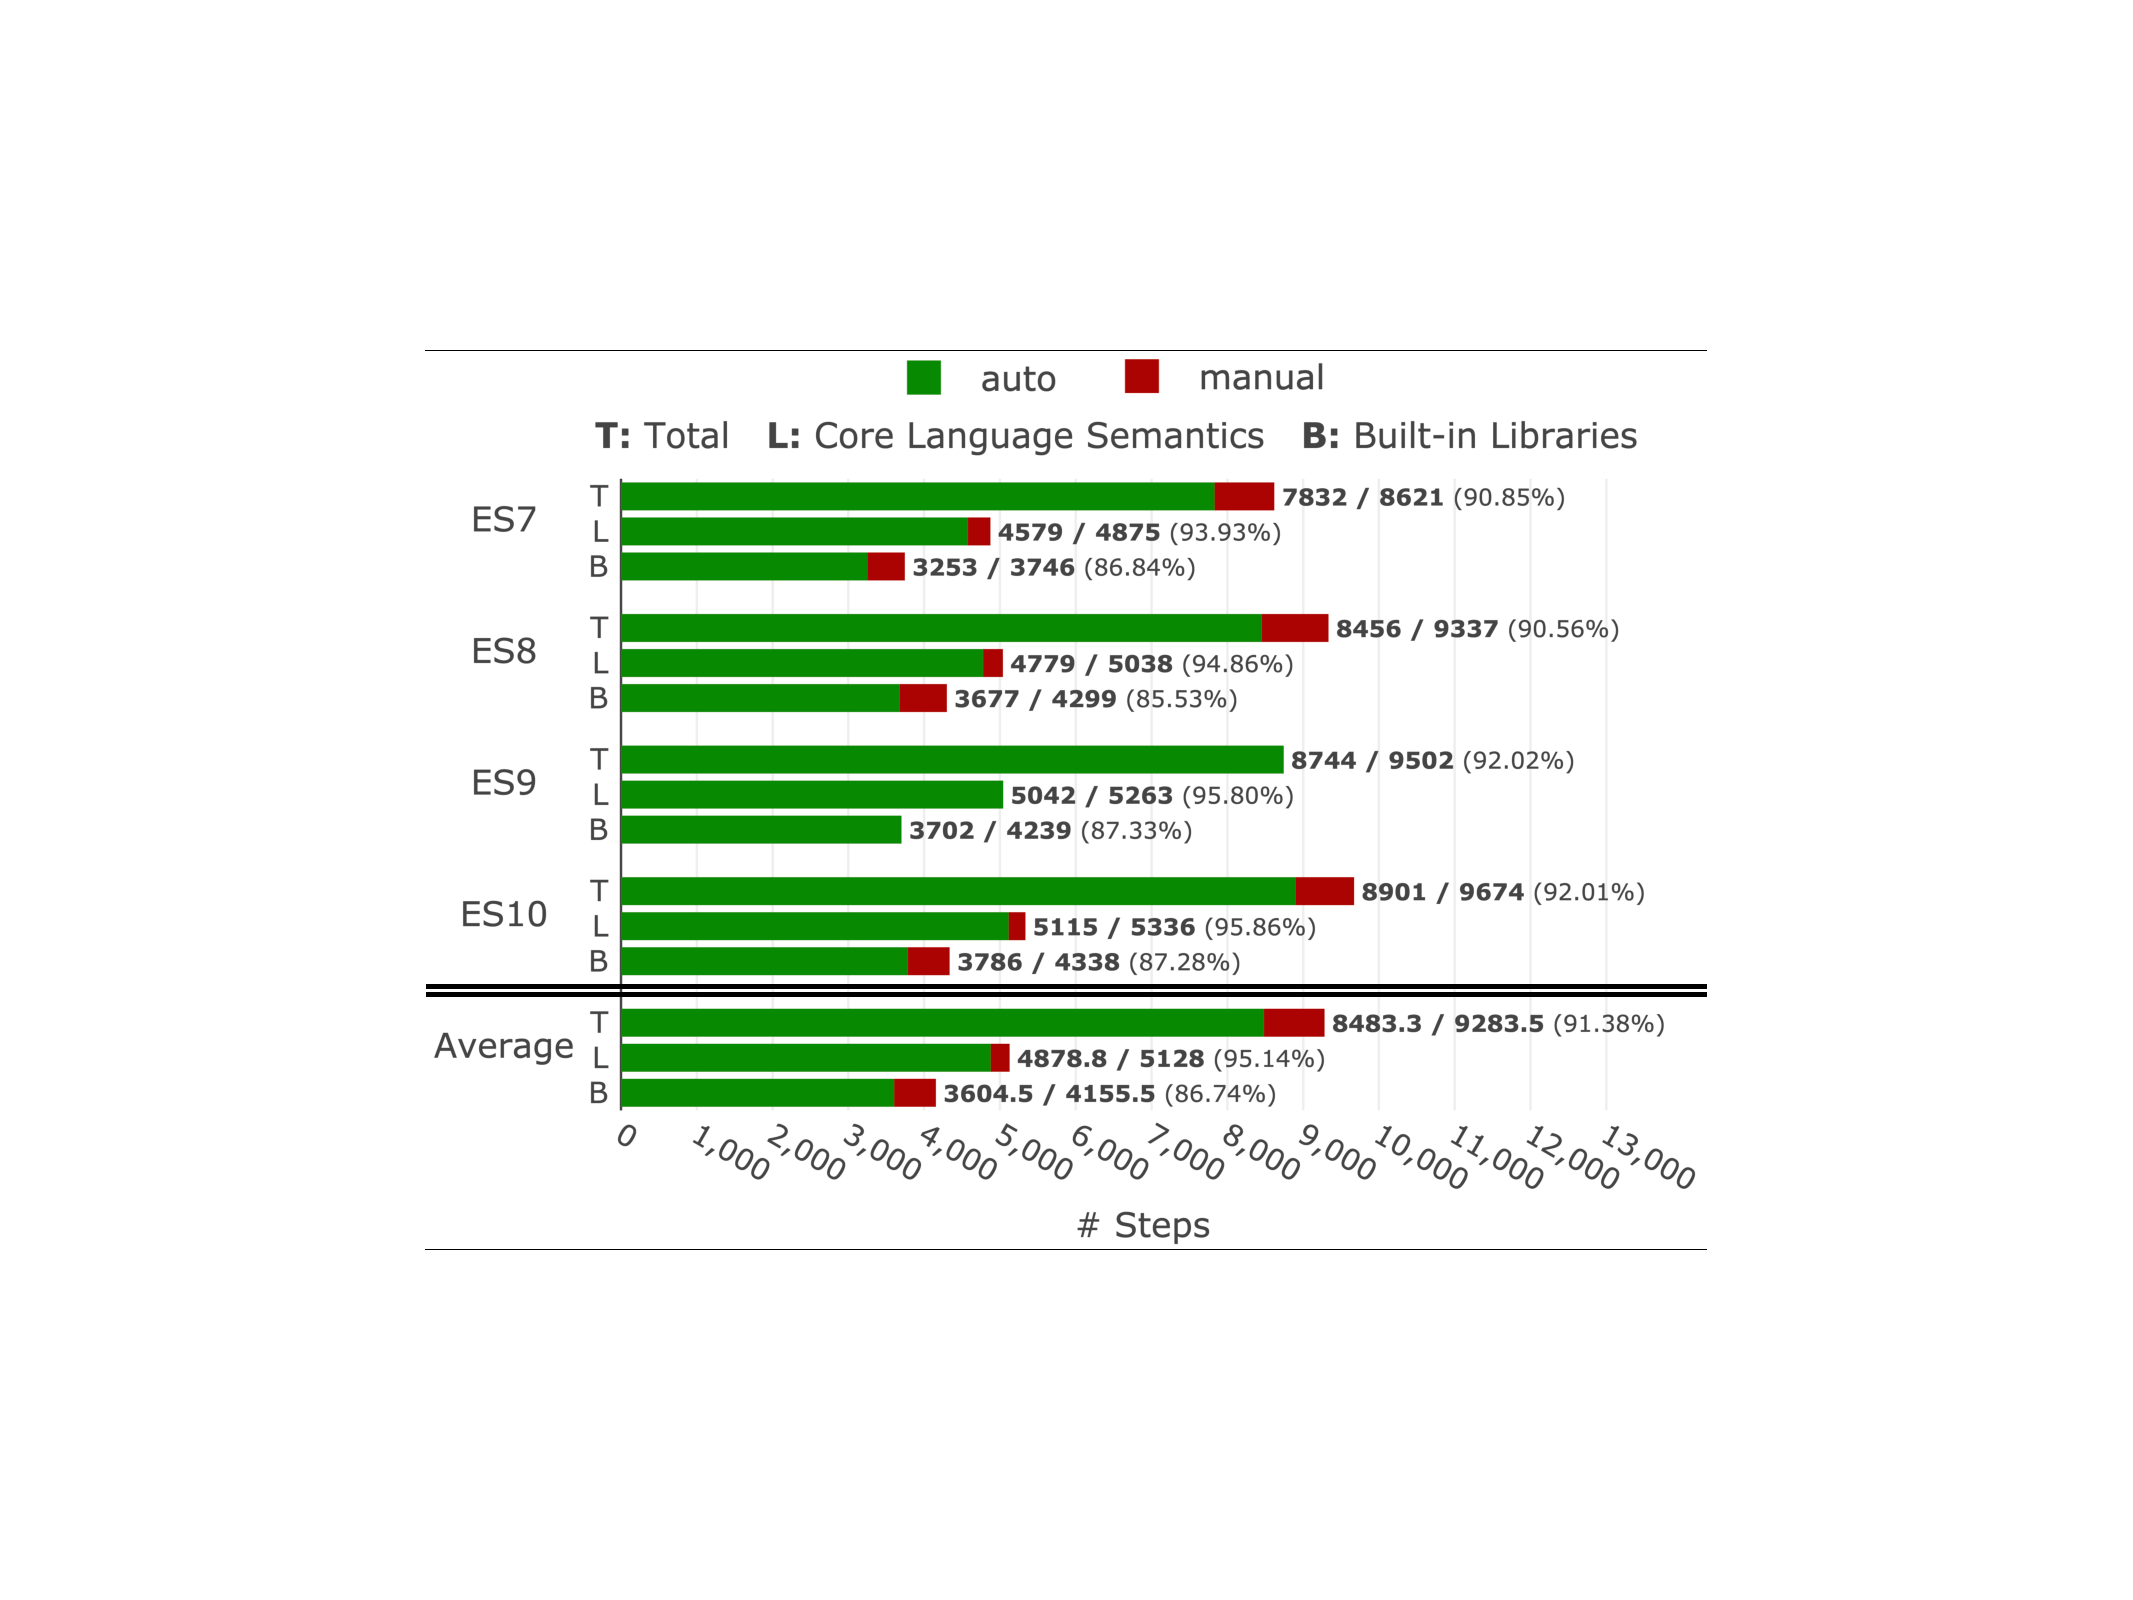
\includegraphics[width=\textwidth]{img/sem-all.pdf}
    \caption{Results for existing versions}
    \label{fig:semantics-all-version}
  \end{subfigure}
  \hfill
  \begin{subfigure}{0.48\textwidth}
    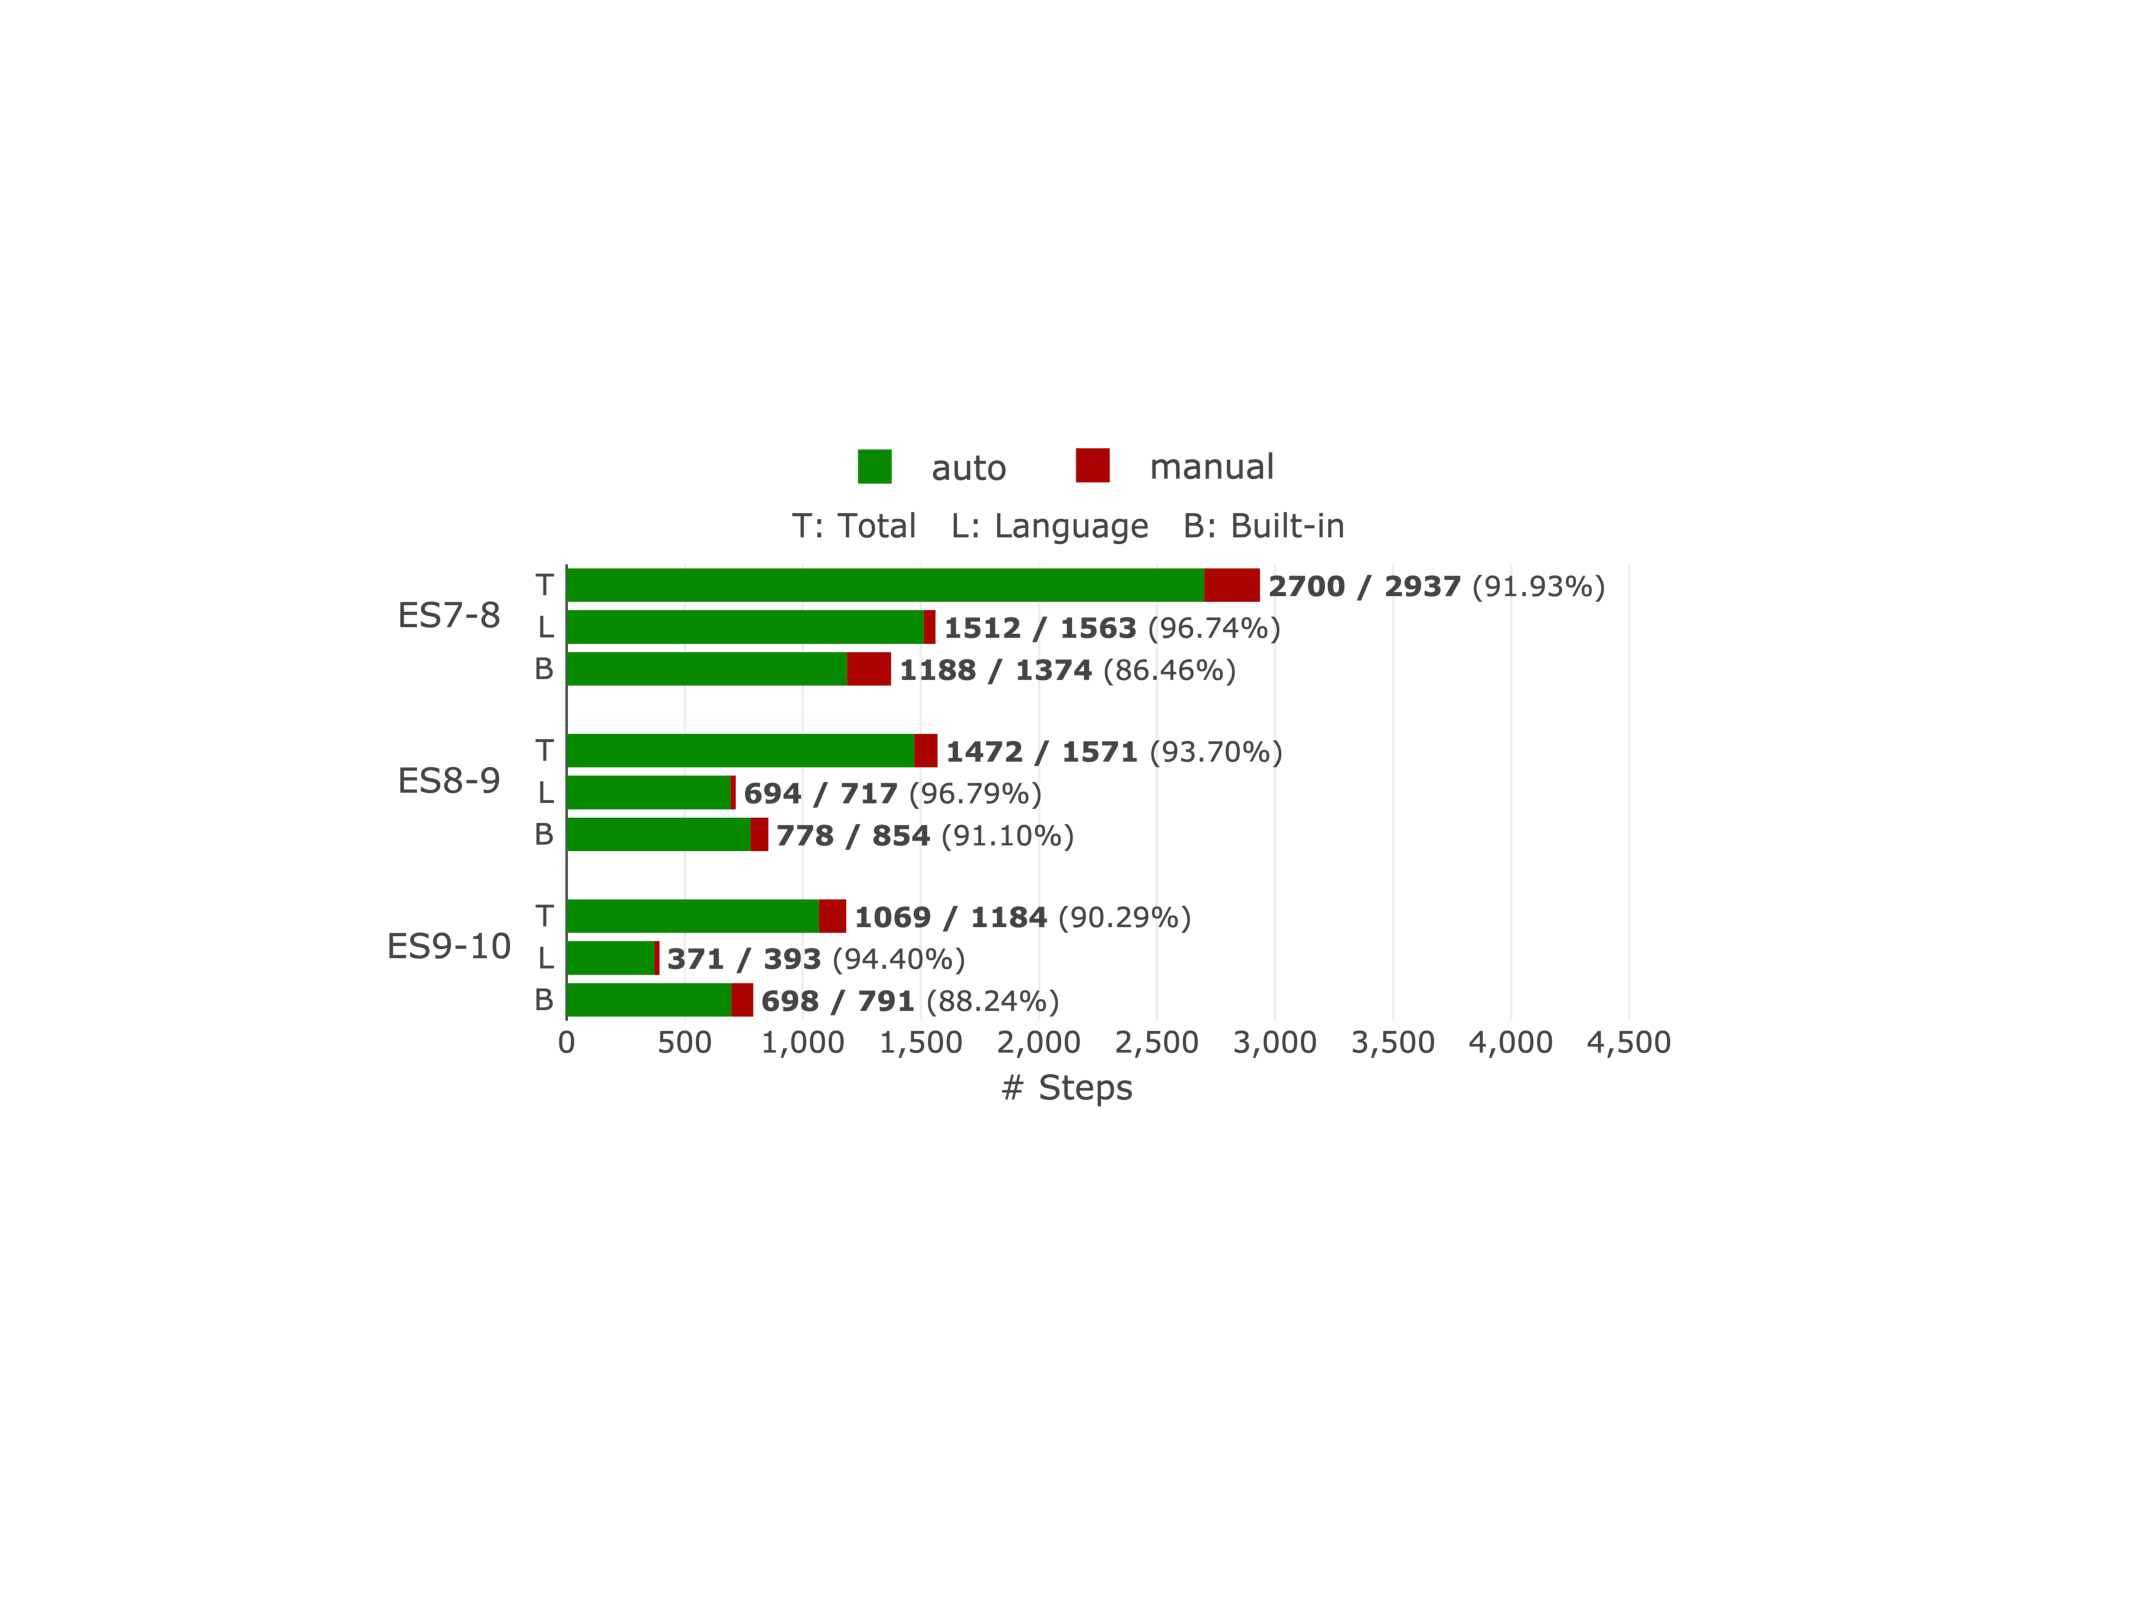
\includegraphics[width=\textwidth]{img/sem-diff.pdf}
    \caption{Results for differences between adjacent versions}
    \label{fig:semantics-all-version-diff}
  \end{subfigure}
  \caption{Number of abstract algorithm steps in specifications, from which
\( \tool \) generated the JavaScript semantics}
  \label{fig:all-version}
\vspace*{-1em}
\end{figure}

For semantics, Figure~\ref{fig:all-version} shows that \( \tool \) automatically
compile algorithm steps to the corresponding \( \ires \) instructions with
\inred{91.60\%} success rate on average for existing specifications, and
\inred{90.43\%} for updates.  ECMAScript abstract algorithms describe not only
core language semantics but also other helper functions of built-in libraries.
Built-in libraries written in more diverse styles in describing their own
specific functionalities.  Thus, built-in libraries have lower success rates
(\inred{86.98\%} for specifications and \inred{86.09\%} for updates) than core
language semantics (\inred{95.35\%} for specifications and \inred{95.25\%} for
updates).

This results show that \( \tool \) effectively reduces the efforts to
extract the syntax and semantics of JavaScript not only for developing
them from scratch, but also for updating existing ones.


\subsection{Check with Tests}\label{sec:check-with-tests}

To define the \textit{first IR-based formal semantics of modern JavaScript}, we
completed missing parts of the AST-IR translator for ES10.  Among \inred{9,674}
steps in ES10, \inred{8,901} steps are automatically compiled via
\textsf{Algorithm Compiler}.  Among the remaining \inred{773} steps, we manually
implemented all remaining language semantics (\inred{221} steps) and essential
parts of built-in libraries (\inred{XX} steps out of \inred{552}) in \inred{XX}
days.  Moreover, we manually implemented the \textsf{Global Setting} as described
in Section~\ref{sec:compiler-impl} for the core language features.  However, we
do not support several minor language features that do not affect the overall
JavaScript semantics critically: non-strict mode codes, modules, early errors
before actual executions, and inessential built-in objects.

Thanks to the executability of our extracted formal semantics, we checked the
semantics with Test262, the official conformance test suite provided by TC39.
We fixed version of Test262 as of February 28, 2019 because the ES10 was
branched out with the branch name es2019 in that day.  While it consists of
\inred{XX,XXX} tests, we filtered out \inred{XX,XXX} tests not applicable for
our formal semantics as shown in Table~\ref{table:test262}.  Test262 targets not
only the current official version of ECMAScript but several extensions and
in-progress features. We excluded \inred{X,XXX} tests for such cases to focus on
the semantics of ES10.  Among \inred{XX,XXX} ES10 tests, we also filtered out
\inred{X,XXX} tests using language features not supported by our semantics.

\begin{table*}[t]
  \centering
  \caption{Specification errors and wrong tests in Test262.}
  \label{table:spec-tests-errors}
  \vspace*{-0.5em}
  \small
  \begin{tabular}{|c|c|l|c|c|c|c|c|}
    \hline
    \multicolumn{1}{|c|}{\bf Name} &
    \multicolumn{1}{c|}{\bf Feature} &
    \multicolumn{1}{c|}{\bf Description} &
    \multicolumn{1}{c|}{\bf Known} &
    \multicolumn{1}{c|}{\bf Created} &
    \multicolumn{1}{c|}{\bf Resolved} &
    \multicolumn{1}{c|}{\bf Existed} &
    \multicolumn{1}{c|}{\bf \# Failed Tests} \\\hline

    es10-1 &
    Await &
    \makecell[l]{Passing wrong type of \\ the second argument for {\bf PromiseResolve}.} &
    \textsf{O} &
    2019-02-27 &
    2019-04-13 &
    45 days &
    \inred{XX} \\\hline

    es10-2 &
    IterationKind &
    \makecell[l]{Missing \code{async-iterate} case \\ in the assertion of {\bf
    ForIn/OfHeadEvaluation}.} &
    \textsf{X} &
    2018-02-16 &
    2020-03-25 &
    768 days &
    \inred{XX} \\\hline

    es10-3 &
    Completion &
    \makecell[l]{Not handling abrupt completion \\ in {\bf Evaluation} of {\it
    EqualityExpression}.} &
    \textsf{O} &
    2016-06-01 &
    2019-05-02 &
    1065 days &
    \inred{XX} \\\hline

    es10-4 &
    Function &
    \makecell[l]{No semantics of {\bf IsFunctionDefinition} \\ for
    \code{function(...)\{...\}}.} &
    \textsf{O} &
    2015-10-30 &
    2020-01-18 &
    1541 days &
    \inred{XX} \\\hline

    es10-5 &
    ForOf &
    \makecell[l]{Two semantics of {\bf VarScopedDeclarations} \\ for \code{for
    await(var x of e)\{...\}}.} &
    \textsf{O} &
    2018-02-16 &
    2019-10-11 &
    602 days &
    \inred{XX} \\\hline

    es10-6 &
    Argument &
    \makecell[l]{No semantics of {\bf ExpectedArgumentCount} \\ for the base case
    of {\it FormalParameters}.} &
    \textsf{O} &
    2016-11-02 &
    2020-02-20 &
    1205 days &
    \inred{XX} \\\hline

    es10-7 &
    String &
    \makecell[l]{Wrong use of \code{=} operator in {\bf
    StringGetOwnProperty}.} &
    \textsf{X} &
    2015-06-01 &
    \inred{2019-00-00} &
    \inred{XX} days &
    \inred{XX} \\\hline

    test-1 &
    Global &
    \makecell[l]{Testing implementation-dependent [[Prototype]] \\ of the global
    object.} &
    \textsf{X} &
    \inred{2019-00-00} &
    \inred{2019-00-00} &
    \inred{XX} days &
    10 \\\hline

    bigint-1 &
    UpdateExpression &
    \makecell[l]{Using wrong variable \code{oldvalue} instead of \\
    \code{oldValue} in {\bf Evaluation} of {\it UpdateExpression}.} &
    \textsf{X} &
    2019-09-27 &
    2020-04-23 &
    209 days &
    \inred{XX} \\\hline

    bigint-2 &
    NumberOp &
    \makecell[l]{Using {\bf ToInt32} instead of {\bf ToUint32} \\ in {\bf
    Number::unsignedRightShift}.} &
    \textsf{X} &
    2019-09-27 &
    2020-04-23 &
    209 days &
    \inred{XX} \\\hline

    bigint-3 &
    NumberOp &
    \makecell[l]{Using {\bf ToUint32} instead of {\bf ToInt32} \\ in {\bf
    NumberBitwiseOp}.} &
    \textsf{X} &
    2019-09-27 &
    2020-04-23 &
    209 days &
    \inred{XX} \\\hline

    bigint-4 &
    Number &
    \makecell[l]{Not handling BigInt values in {\bf Number} constructor.} &
    \textsf{O} &
    2019-09-27 &
    2019-11-19 &
    53 days &
    \inred{XX} \\\hline

  \end{tabular}
\end{table*}

\begin{table}[t]
  \centering
  \caption{Excluded tests in Test262}
  \label{table:test262}
  \vspace*{-0.5em}
  \small
  \begin{tabular}{lr}\toprule
    \belowrulesepcolor{gainsboro}
    \rowcolor{gainsboro} \textbf{All Test262 Tests} & \inred{\textbf{XX,XXX}}\\
    \aboverulesepcolor{gainsboro}\midrule
    Annexes & \inred{XXX}\\\hdashline
    Internationalization & \inred{XXX}\\\hdashline
    In-progress features & \inred{X,XXX}\\\midrule
    \belowrulesepcolor{gainsboro}
    \rowcolor{gainsboro} \textbf{ES10 Tests} & \inred{\textbf{XX,XXX}}\\
    \aboverulesepcolor{gainsboro}\midrule
    Non-strict modes & \inred{X,XXX}\\\hdashline
    Modules & \inred{X,XXX} \\\hdashline
    Early errors & \inred{X,XXX} \\\hdashline
    Inessential built-in objects & \inred{X,XXX} \\\midrule
    \belowrulesepcolor{gainsboro}
    \rowcolor{gainsboro} \textbf{Applicable Tests} & \inred{\textbf{XX,XXX}}\\
    \aboverulesepcolor{gainsboro}\midrule
    Passed tests & \inred{XX,XXX} \\\hdashline
    Failed tests & \inred{XXX} \\\bottomrule
  \end{tabular}
  \vspace*{-2em}
\end{table}

For \inred{XX,XXX} applicable tests, the synthesized JavaScript parser
successfully parses all tests but \inred{XXX} tests are failed to be executed
because of the different semantics between ECMAScript and official tests.  Based
on the failed tests, we found 7 specification errors in ES10 and 10 wrong tests
in Test262 as described in Table~\ref{table:spec-tests-errors}.  For example,
the specification error es10-1 is related to the JavaScript Await.  The {\bf
PromiseResolve (C, x)} algorithm creates a new Promise object using a given
constructor {\bf C} and resolved with a given value {\bf x}.  However, a
specification update added three invocations of {\bf PromiseResolve} with a list
of values for {\bf x} in February 27, 2019.  This error exists in 45 days until
April 13, 2019 and fails \inred{XX} tests for ES10 in Test262.  For other cases,
es10-2 arises because of the wrong assertion. es10-3 and es10-7 arise because
contributors misunderstood the meaning of abrupt completion and \code{=}
operator for numbers, respectively.  es10-4, es10-5, and es10-6 are
specification errors that miss or define twice specific corner cases of
semantic.  For example, es10-4 is an error that does not define the {\bf
IsFunctionDefinition} algorithm for unnamed functions such as
\code{function(){}}.  For these seven specification errors, they existed in ES10
in \inred{XXX} days on average.  Besides, two errors es10-2 and es10-7 are even
not known before we reported to TC39.

For tests in Test262, we found 10 wrong tests categorized in test-1 and they are
related to the JavaScript global object. The [[Prototype]] internal property of
the global object is fully implementation dependent thus the official tests
should not check its attributes.  However, 10 tests assumes that [[Prototype]]
of the global object is a prototype chain starts with \code{Object.prototype}.
They violate the implementation dependent semantics of ES10.  Moreover, they
existed in Test262 in \inred{XXX} days.

After resolving above specification errors in ES10, we extracted formal
semantics from the revised specification again. The revised formal semantics of
ES10 passed all \inred{XX,XXX} applicable tests in Test262.  We believe that our
tool can assist to check and find bugs in ECMAScript by generating executable
formal semantics and executing it with tests in Test262.


\subsection{Forward Compatibility}

We show the forward compatibility of \( \tool \) by applying it to the proposals
that are ready for inclusion in the next ECMAScript (ES11, 2020). Because
ECMAScript administered as an open-source project, various proposals for new
language features are available with their own specification changes and tests.
A separate repository~\cite{proposals} maintains such proposals with six
different stages: Stage 0 to Stage 3, Finished, and Inactive.  Each proposal
starts with Stage 0, and the TC39 committee regularly examines Stage 3 proposals
to decide their next stages.  If a proposal is confirmed, the committee changes
its stage to Finished and integrates it into the next version of ECMAScript.
Otherwise, the committee changes its stage to Inactive.  Among them, we applied
\( \tool \) to all Finished proposals decided to be included in ES11.

\begin{table}[t]
  \centering
  \caption{Evaluation result of \( \tool \) for Finished stage proposals that
  will be included in ES11.}
  \label{table:spec-prop-result}
  \vspace*{-0.5em}
  \small
  \begin{tabular}{c?r|r?r?r}
    \hline
    \multicolumn{1}{c?}{\multirow{2}{*}{\bf Name}} &
    \multicolumn{2}{c?}{\bf \( \Delta \) \# Prod.} &
    \multicolumn{1}{c?}{\multirow{2}{*}{\bf \( \Delta \) \# Steps}} &
    \multicolumn{1}{c}{\multirow{2}{*}{\bf \# Tests}} \\\cline{2-3}

    &
    \multicolumn{1}{c|}{\bf Lex.} &
    \multicolumn{1}{c?}{\bf Syn.} &
    &\\\hline\hline

    \code{matchAll} of \code{String} &
    0 &
    0 &
    9/9 &
    5/5\\\hline

    \code{import()} &
    0 &
    2 &
    22/23 &
    0/0\\\hline

    \code{BigInt} &
    4 &
    0 &
    258/323 &
    \inred{207}/207\\\hline

    \code{Promise.allSettled} &
    0 &
    0 &
    79/85 &
    50/50\\\hline

    \code{globalThis} &
    0 &
    0 &
    1/1 &
    1/1\\\hline

    \code{for-in} mechanics &
    0 &
    0 &
    36/37 &
    0/0\\\hline

    Optional Chaining &
    3 &
    3 &
    72/74 &
    19/19\\\hline

    Nullish Coalescing Op. &
    1 &
    4 &
    10/10 &
    21/21\\\hline

    \code{import.meta} &
    0 &
    2 &
    15/15 &
    0/0\\\hline

    {\bf Total} &
    8 &
    11 &
    502/577 &
    \inred{303}/303\\\hline
  \end{tabular}
\end{table}

Table~\ref{table:spec-prop-result} shows the result of applying \( \tool \) to 9
Finished proposals for ES11.  For all proposals, \inred{XX} lexical and
\inred{XX} syntactic productions are modified and \( \tool \) successfully
updated the changes to the synthesized JavaScript parser.  The updated parser
parses all applicable tests for all proposals.  For abstract algorithms,
\inred{XXX} steps out of \inred{XXX} steps are automatically converted to the
corresponding \( \ires \) instructions by the algorithm compiler without
changing of the compile rules.  Thus, our tool has \inred{XX.XX\%} success rate
on average for future proposals.  Similar with
Section~\ref{sec:check-with-tests}, we manually implemented missing part of the
AST-IR translator for each Finished proposal and checked each extracted
semantics with official tests.  Each of them passed all applicable tests except
the semantics for \code{BigInt} proposal.  It fails \inred{XX} tests out of 207
applicable tests.

Based on the failed tests, we found three undiscovered specification errors
(bigint-1, bigint-2, and bigint-3), and one reported error (bigint-4) in the
BigInt proposal as described in Table~\ref{table:spec-tests-errors}.  All of
them were confirmed by TC39 and will be fixed in the next release.  The BigInt
proposal added a new type of primitives BigInt and unified the type with
original Number type to Numeric types.  Thus, it not only added new
algorithms for BigInt but also modified all existing algorithms related to
number values.  The error bigint-1 is just a simple misuse of the variable
\code{oldValue} in {\bf Evaluation} of {\it UpdateExpression}. bigint-2 and
bigint-3 break the backward compatibility because of the incorrectly mixed uses
of {\bf ToInt32} and {\bf ToUint32} algorithms in unsigned right shift operators
and bitwise operators, respectively. The last one bigint-4 arises because the
Number constructor does not consider BigInt primitives.  On average, ECMAScript
included these four specification errors in \inred{XXX} days.

After fixing all specification errors, we extracted the semantics for the BigInt
proposal again.  The updated semantics passed all 207 applicable tests.  Thus,
\( \tool \) also correctly extract IR-based semantics from future proposals.
